\let\negmedspace\undefined
\let\negthickspace\undefined
\documentclass[journal]{IEEEtran}
\usepackage[a5paper, margin=10mm, onecolumn]{geometry}
%\usepackage{lmodern} % Ensure lmodern is loaded for pdflatex
\usepackage{tfrupee} % Include tfrupee package

\setlength{\headheight}{1cm} % Set the height of the header box
\setlength{\headsep}{0mm}     % Set the distance between the header box and the top of the text

\usepackage{gvv-book}
\usepackage{gvv}
\usepackage{cite}
\usepackage{amsmath,amssymb,amsfonts,amsthm}
\usepackage{algorithmic}
\usepackage{graphicx}
\usepackage{textcomp}
\usepackage{xcolor}
\usepackage{txfonts}
\usepackage{listings}
\usepackage{enumitem}
\usepackage{mathtools}
\usepackage{gensymb}
\usepackage{comment}
\usepackage[breaklinks=true]{hyperref}
\usepackage{tkz-euclide} 
\usepackage{listings}
% \usepackage{gvv}                                        
\def\inputGnumericTable{}                                 
\usepackage[latin1]{inputenc}                                
\usepackage{color}                                            
\usepackage{array}                                            
\usepackage{longtable}                                       
\usepackage{calc}                                             
\usepackage{multirow}                                         
\usepackage{hhline}                                           
\usepackage{ifthen}                                           
\usepackage{lscape}
\usepackage{circuitikz}
\tikzstyle{block} = [rectangle, draw, fill=blue!20, 
    text width=4em, text centered, rounded corners, minimum height=3em]
\tikzstyle{sum} = [draw, fill=blue!10, circle, minimum size=1cm, node distance=1.5cm]
\tikzstyle{input} = [coordinate]
\tikzstyle{output} = [coordinate]


\begin{document}

\bibliographystyle{IEEEtran}
\vspace{3cm}

\title{4.10.9}
\author{EE25BTECH11009 - Anshu Kumar Ram }
\maketitle
% \newpage
% \bigskip
{\let\newpage\relax\maketitle}

\renewcommand{\thefigure}{\theenumi}
\renewcommand{\thetable}{\theenumi}
\setlength{\intextsep}{10pt} % Space between text and floats


\numberwithin{equation}{enumi}
\numberwithin{figure}{enumi}
\renewcommand{\thetable}{\theenumi}
\textbf{Question}:\\
Find the equation of the plane passing through the line of intersection of the planes 
\begin{align}
\vec{r} \cdot (\hat{i} + 2\hat{j} + 3\hat{k}) - 4 &= 0, \\
\vec{r} \cdot (2\hat{i} + \hat{j} - \hat{k}) + 5 &= 0
\end{align}
and which is perpendicular to the plane 
\begin{align}
\vec{r} \cdot (5\hat{i} + 3\hat{j} - 6\hat{k}) + 8 &= 0.
\end{align}
\solution \\
Given -
the equation of the plane passing through the line of intersection of the planes
\begin{align}
\vec{r}\cdot \myvec{1 \\ 2 \\ 3} = 4 
\end{align}
and 
\begin{align}
\vec{r}\cdot \myvec{2 \\ 1 \\ -1} + 5 = 0
\end{align}
and perpendicular to the plane
\begin{align}
\vec{r}\cdot \myvec{5 \\ 3 \\ -6} + 8 = 0
\end{align}



The required plane can be written as a linear combination of the first two planes:
\begin{align}
(\vec{n}_1 + \lambda \vec{n}_2)^T\vec{r} = c_1 + \lambda c_2
\end{align}
where
\begin{align}
\vec{n}_1 = \myvec{1 \\ 2 \\ 3}, \quad c_1 = 4
\end{align}
\begin{align}
\vec{n}_2 = \myvec{2 \\ 1 \\ -1}, \quad c_2 = -5
\end{align}

Thus, the normal vector of the required plane is
\begin{align}
\vec{n} = \vec{n}_1 + \lambda \vec{n}_2
\end{align}

Since the plane is perpendicular to 
\begin{align}
\vec{r}\cdot \myvec{5 \\ 3 \\ -6} + 8 = 0
\end{align}
we must have
\begin{align}
\vec{n}^T \vec{n}_3 = 0, \quad \vec{n}_3 = \myvec{5 \\ 3 \\ -6}
\end{align}

That is,
\begin{align}
	(\vec{n}_1 + \lambda \vec{n}_2)^{\top} \vec{n}_3 = 0
\end{align}

Substituting values,
\begin{align}
\myvec{1 && 2 && 3} \myvec{5 \\ 3 \\ -6} + \lambda \myvec{2 && 1 && -1} \myvec{5 \\ 3 \\ -6} = 0
\end{align}
\begin{align}
-7 + 19\lambda = 0 \implies \lambda = \frac{7}{19}
\end{align}

Thus,
\begin{align}
\vec{n} = \vec{n}_1 + \frac{7}{19}\vec{n}_2 = \frac{1}{19}\myvec{33 \\ 45 \\ 50}
\end{align}

Also,
\begin{align}
c = c_1 + \lambda c_2 = 4 + \frac{7}{19}(-5) = \frac{41}{19}
\end{align}

Multiplying through by $19$, the required plane is
\begin{align}
\myvec{33 & 45 & 50}\vec{r} = 41
\end{align}

\textbf{Final Answer:}
\begin{align}
33x + 45y + 50z = 41
\end{align}




\begin{figure}[h!]
    \centering
    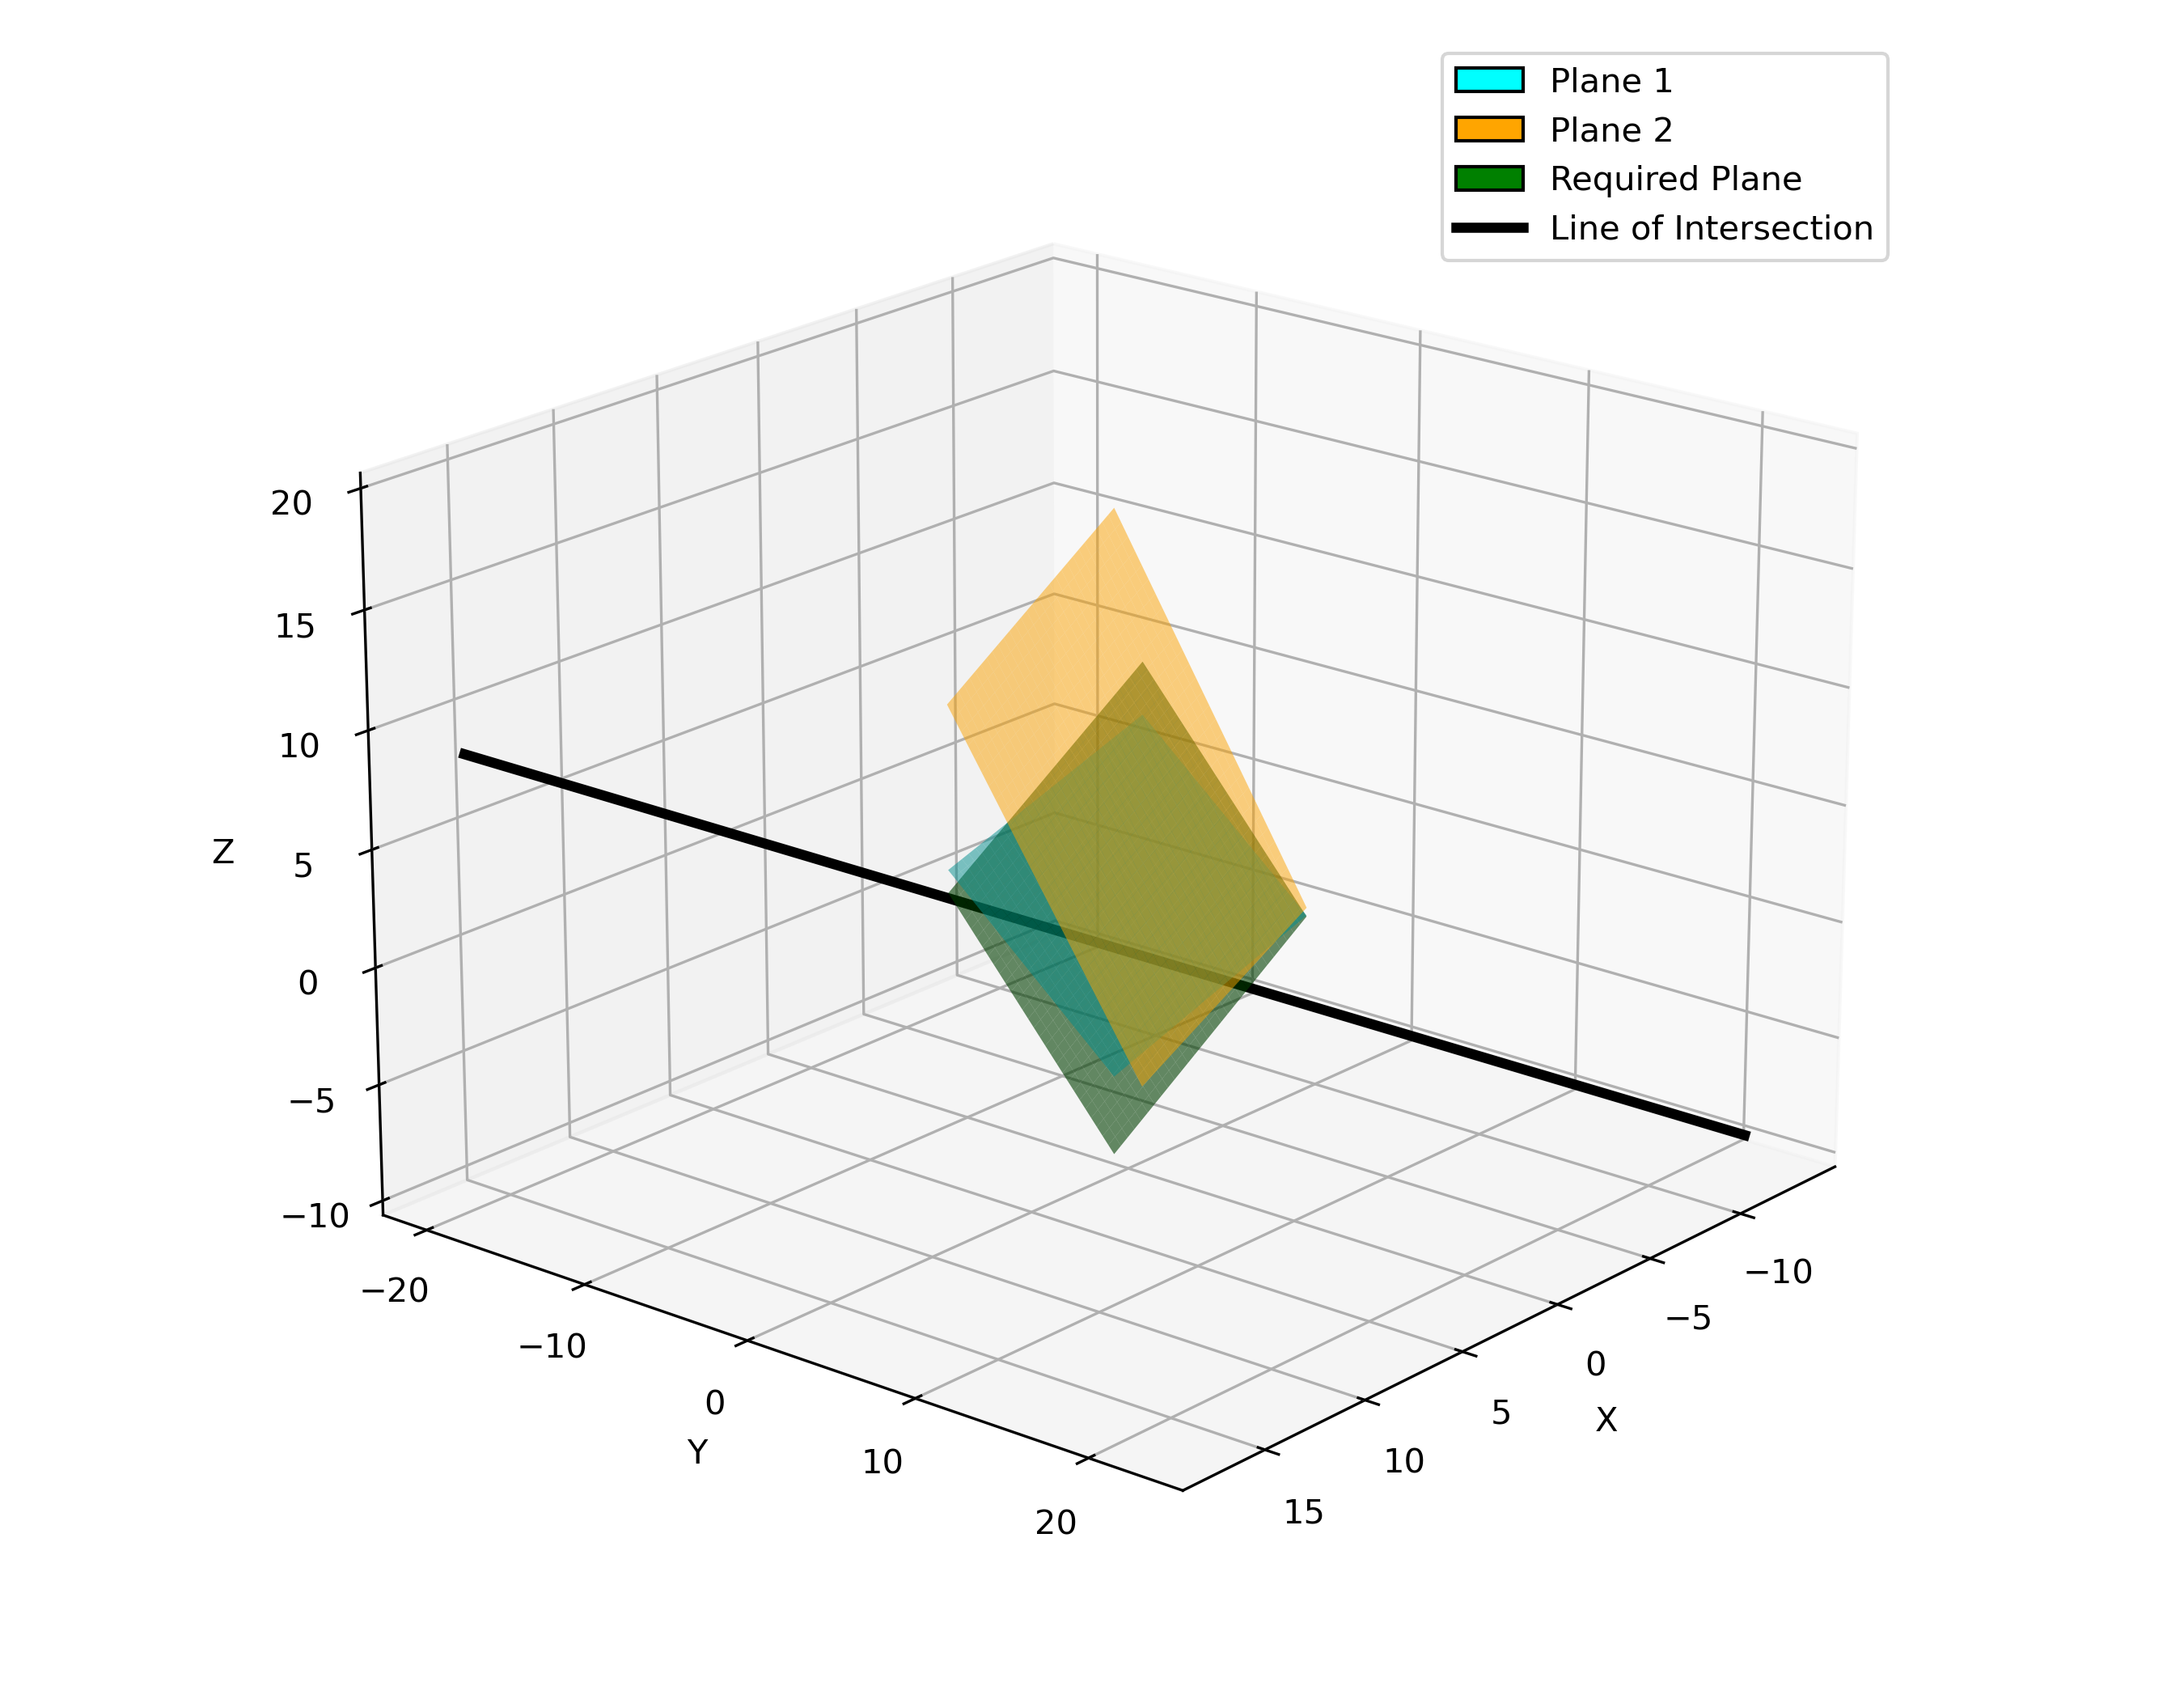
\includegraphics[height=0.5\textheight, keepaspectratio]{figs/Figure_1.png}
    \label{figure_1}
\end{figure}

\end{document} 
